\subsection{Actores y roles}
\begin{itemize}
\item \textbf{Administrador:} Es la cabeza de la empresa y el punto de control en el maximo de procesos que puede involucrarse, por esto la desiciones de la empresa pasan todas por él. Tambien se preocupa del abastecimiento de insumos y de la mantencion de los recursos. 

\item \textbf{Vendedoras:} En la sala de venta se preocupan de ser el primer contacto con los clientes, dandole accesos a los productos y cuantificandolos en dinero para que el cliente pueda pagar.

\item \textbf{Cajero:} La unica tarea de esta persona es cobrar el dinero en la sala  de venta. Siendo  la persona de confianza en la sala de venta del administrador, pero sin tener poder de desición en este lugar.

\item \textbf{Repartidores:} Se encargan de ser el nexo entre la panadería y la distribución de pan a mayor escala. Distribuyen el pan, cobran en algunos casos y tienen la potestad de poder hacer nuevos clientes de gran escala.
\end{itemize}

\subsection{Modelos de procesos nivel 1}
La panadería Rodenas se dedica a la fabricación, venta y distribución de pan y reposteria. A nivel macro todo empieza con una solicitud diaria que da el inicio al trabajo, pasando por el proceso de fabricación de pan (Producción de pan) y el proceso de fabricación de reposteria (Producción de reposteria), una vez terminados estos procesos pueden pasar a la Distribución o Ventas dependiendo de que prioridad tiene cada uno en el mismo momento, esto pasa por una decisión del Administrador. Después tenemos el proceso Ventas que se encarga de la venta del pan, venta de resposteria y atención al cliente, pero puede suceder que el proceso de Ventas antes que termine se vea entorpecido por si falta o no pan o reposteria, aquí es donde vuelve al proceso de Producción y se realiza nuevamente el flujo. Paralelo a este proceso tenemos Distribución, que es el encargado de tomar los pedidos durante el día y terminar el flujo diario.

\begin{center}
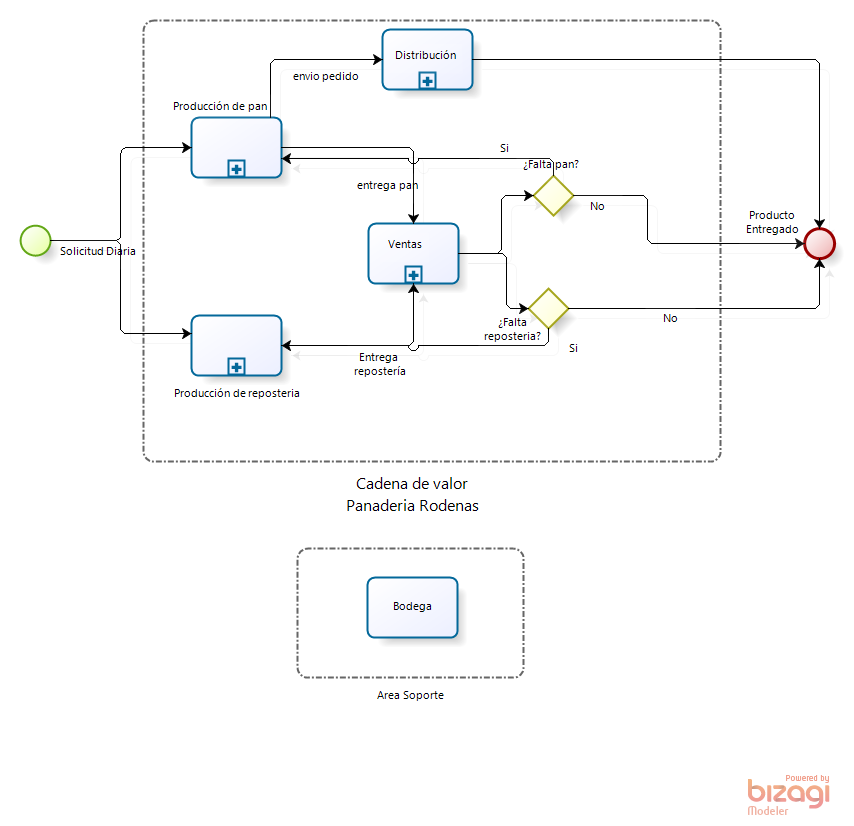
\includegraphics[width=15cm]{./imagenes/Macro_proceso.png}\\
Figura 1: Macro-proceso de panadería Rodenas.
\end{center}
\subsection{Descripción de modelos de procesos nivel 1} 
